% !TEX root = ../CedricDe Schepper2023_Thesis.tex

\section{Related Work}\label{sec:related-work}

This section details different types of algorithms researched to solve the timetabling problem. Additionally, it will also go over several benchmarks used to compare these algorithms.
%TODO expand on this


% \begin{description}
%     \item [Integer Programming] Integer Programming tries to solve an optimisation by minimising or maximising the problem's objective function. Fundamentally, some or all required variables are constrained to integers. Since integer programming makes use of an exhaustive search process, the search space must be reduced as much as possible to reduce the run time.
%     \item [Simulated Annealing] Simulated annealing\cite{kirkpatrick1983} makes use of a temperature variable which describes the level of randomness present in the acceptance of a new solution. After generating an initial solution, newly obtained solutions are accepted based on the change in objective function and current temperature. Over time the temperature cools down which reduces the amount of randomness.
%     \item [Adaptive Large Neighbourhood Search] Adaptive large neighbourhood search (ALNS) \cite{ropke2006} works by generating new solutions by constantly making changes to the current solution in order to explore the neighbourhood space. These changes are obtained by removing part of the variables and then reintroducing new values in order to generate neighbours. ALNS is considered adaptive since it keeps track of the performance of certain operations and adjusts its parameters accordingly. The use of ALNS for exam timetabling so far has been limited.
%     \item [Genetic Algorithms] Genetic algorithms (GA) \cite{Holland1975} are based on the process of natural selection witnessed in nature. They work by generating an initial set or population of possible solutions. Iteratively, a new population will be formed by selecting the fittest (best) solutions and combining two solutions to create a new generation of solutions.
%     \item [Particle Swarm Optimisation] Particle swarm optimisation (PSO) \cite{kennedy1995} is derived from the behaviour by collective species as seen in fish schools and bird flocks. A swarm of particles (see fish or bird), representing solutions, moves through the search space at a certain speed and direction.
%     \item [Honey-Bee Mating Optimisation] Honey-bee mating optimisation algorithms (HBMO) \cite{abbas2001} are based on the mating of honey-bees as witnessed in nature. During the mating procedure, the queen representing the current best solution is able to mate with other bees in order to produce new solutions.
%     \item [Great Deluge] Great deluge algorithms (GD) \cite{dueck1993} are based on the principle where an increasing water level is used to represent the allowed threshold. Only a solution that is superior in comparison with that threshold is accepted.
%     \item [Hyper-heuristics] Hyper-heuristics\cite{cowling2001} are designed to be problem-independent meaning no domain expertise and customisation is needed to be successfully applied to different problems. These heuristics utilise the heuristic the most optimal for the given problem.
% \end{description}
From previous surveys collecting different algorithms used to solve the examination timetabling problem, we identify several classes for optimisation methods, all with their own unique characteristics \cite{joo2021, kristiansenSurvey2013, chen2021, rong2009}. Papers focusing on single algorithms were mainly found by conducting backward snowballing. From the initial survey papers, relevant references were considered for further review. Occasionally, Google Scholar was used to look for additional research papers on a specific topic. From these papers, we cover the following optimisation method classes are covered in this section:
\begin{description}
\item [Single Solution-based Meta-heuristics] \hfill \\
Single Solution-based Meta-heuristics are also commonly referred to as Local Search methods \cite{lin1973}. These heuristics first generate an initial solution. Afterwards, small changes are continuously applied to the solution using a specific strategy in order to traverse the search space. 

They can often be divided into either one-stage or two-stage algorithms \cite{lewis2008}. One-stage methods attempt to satisfy both the hard and soft constraints during the same stage. Two-stage approaches initially only take the hard constraints into account in order to generate a feasible solution. Afterwards, the second phase attempts to optimise the solution by adding the soft constraints. Since Local Search methods only accept a solution when it is better than the previous one, encountering a worse solution blocks them from progressing. This means that Local Search requires strategies in order to escape local optima and keep improving the solution. 

% discuss the many parameters?


\item [Population-based Meta-heuristics] \hfill \\
Instead of applying a meta-heuristic on a single solution, Population-based meta-heuristics maintain a set of solutions, called a population. Every iteration, a new population is generated by applying meta-heuristics. These methods offer the advantage over single solution-based methods that multiple solutions are presented during the final iteration. Another difference is that they prioritise exploration of the search space while single solution-based methods focus more on exploitation of their solution  \cite{kohshori2012}. However, this exploration does come at the cost of an increase in run time due to a larger amount of operations applied at each iteration.

\item [Exact Methods]  \hfill \\
Exact methods constrain the problem by defining a linear objective function and force some or all parameters to be integers. Since these methods make use of an exhaustive search process, the search space must be reduced as much as possible to decrease the run time. Unlike heuristics, exact methods can provide upper and lower bounds of the objective function and thus provide proof of optimality. Fundamentally, some or all required variables are constrained to integers. 

\item [Hyper-heuristics] \hfill \\
Hyper-heuristics\cite{cowling2001, burke2013} are designed to be problem-independent meaning no domain expertise and customisation is needed to be successfully applied to different problems. They utilise the most optimal heuristic for the given problem.

\end{description}

\subsection{Standardised data sets and benchmarks} \label{benchmarks}

Even though the timetabling problem has been tackled in many research papers, Ceschia et al.\cite{ceschia2022} state that many of the initial benchmarks are not relevant anymore. They observe that many papers do not provide the data, source code, or solutions used. This makes it impossible to reproduce the presented results. Additionally, many of the problems researched are unique to specific institutions, reducing the amount of relevant observations that can be made from the results. However, effort has been put into standardising the timetabling problems into data sets that can be used to accurately compare different heuristics. The agreement regarding the need for benchmarks dates back to the 'first International Conference on the Practice and Theory of Automated Timetabling' in 1995 \cite{cumming1995}. Most of the current benchmarks available come from competitions like the International Timetabling Competition.

An early formulation for university exam timetabling was presented by Carter et al. \cite{carter1996}. They initially introduced 13 exam timetabling data sets for several institutions, commonly referred to as the Toronto or Carter benchmarks. Additional instances have been made available over time \cite{bellio2021}. The data behind this format is implemented as a binary enrolment matrix, showing for each exam and student whether the student is enrolled for that exam. The objective function to compare solutions for this benchmark is based on the distance between exams and the amount of common students. The penalty for two exams with $k$ common students at a distance of $i$ periods was calculated as $k*w_{i}$. The values for $w_1$, $w_2$, $w_3$, $w_4$, and $w_5$ were set as $16$, $8$, $4$, $2$, and $1$, respectively. While this benchmark is still being used to compare heuristics, the simplification of several common constraints means that it less suitable to apply on real-world scenarios. For example, the benchmark is considered to be uncapacitated. This means that exam rooms are not taken into account when generating timetables. Since constraint 2 determines room capacity to be nonnegotiable, our timetabling problem does not fit in this format.

A later examination timetabling formulation was proposed for ITC-2007 by McCollum et al. \cite{mccollum2007}. This formulation is more advanced than the one proposed by Carter et al., taking more constraints into account. New constraints include the addition of exam rooms and more strict penalties related to the distance of scheduled exams. Initially, a data set of 12 instances was released for the competition but more real-world instances have been translated to the format over time \cite{parkes2010}, as well as the implementation of a generator to create artificial instances \cite{battistutta2017}.

Other common benchmarks focus on either the high school or university course scheduling problem. For example, Post et al. \cite{post2012} were the first to propose a standardised format for  high school timetabling. They developed XHSTT, an XML format to be used in solution benchmarks. Several data sets have been made available at \url{https://www.utwente.nl/en/eemcs/dmmp/hstt/}.
Additionally, this format has been used as the target for the third International Timetabling Competition in 2011. Unfortunately, university exam timetabling problems are often incompatible with course timetabling formats due to differences in constraints and schedule characteristics. Other examples include the Curriculum-based Course Timetabling \cite{gaspero2007} and Post-Enrolment Course Timetabling\cite{lewis2007} formats, both used for ITC-2007.

These problem formulations provide valuable contributions in standardising the timetabling research, allowing for easier comparison between algorithms and verification of solutions. However, the uniqueness of the use case for the University of Antwerp makes using these benchmarks infeasible. As a result, the comparison of the quality of generated solutions can only be made against those produced manually by the university's administration.

\subsection{Single Solution-based Meta-heuristics}

Single Solution-based Meta-heuristics or Local Search methods start from an initial solution. Generally, this solution is generated randomly or using a greedy algorithm, but other techniques can also be used. After that, Local Search starts exploring the search space by calculating the neighbourhood of its current solution and picking a neighbour as its new solution. Different versions of Local Search employ their own technique for selecting the neighbour and for determining when to stop the search. The objective function is used to estimate the quality of each solution, with Local Search attempting to minimise this objective.

\subsubsection{Tabu Search}

Tabu Search \cite{glover1993} is based on Local Search \cite{lin1973}, meaning it traverses the possible search space by performing local changes to the current solution. Since Local Search will only accept improving solutions, this traversal can end up being stuck in local optima. Tabu Search differs from Local Search by relaxing this rule and also accepting worsening solutions. This relaxation allows for more exploration, which results in Tabu Search being able to more easily escape local optima. Additionally, Tabu Search maintains a memory structure to avoid changes being reversed. The usage of short- to long-term memory is based on the assumption that optimisation techniques must incorporate memory to qualify as intelligent and that a bad strategic choice is superior to a good random choice\cite{glover1999}. This memory structure is implemented by maintaining a tabu list which contains the x most recent changes performed. A change is considered ‘tabu’ if it is present within the tabu list.

Alvarez-Valdes et al. \cite{alvarez1997} propose a two-phased Tabu Search implementation in order to solve the university exam timetabling problem. During the first phase, the emphasis is on satisfying the hard constraints. More specifically, they attempt to reduce the amount of occurrences where a student has two exams on the same day. Optimally, this initialisation phase would return a solution that is already feasible. The second phase can be considered an optimisation phase, which tries to satisfy the soft constraints as much as possible and thus attempts to spread the exams as best as possible. They used this algorithm on real-world data sets of the University of Valencia, and compared it with the manually designed exam schedules. They conclude that the generated schedules are superior for all data sets.

Di Gaspero and Schaerf \cite{gaspero2001} adapt the original Tabu Search method by proposing changes to the tabu list and stopping criterion. Instead of keeping a fixed tabu list size, each move is assigned a number of iterations that the move is considered tabu. Additionally, the algorithm will terminate after a fixed amount of iterations without improvement. When comparing their results with the Carter benchmarks, they note that Tabu Search provides comparable performance with the benchmarks.

Chu and Fang \cite{Chu2000} made a comparison between using Genetic Algorithms versus Tabu Search to obtain timetables. For all of their different analyses, the Tabu Search implementation was able to outperform their Genetic Algorithm version, both on the quality of the solution and the computational time needed to converge. However, a redeeming quality of Genetic Algorithms is that they are able to produce several near optimal solutions in one go while Tabu Search implementations are limited to a single solution. 
% TODO remove or not
Colorni et al. \cite{colorni1999} apply Tabu Search, Simulated Annealing, and Genetic Algorithms on the high school timetabling problem for an Italian high school. They conclude that Tabu Search outperforms both competitors in generating quality timetables for their use case.


\subsubsection{Simulated Annealing}

Aycan and Ayav \cite{aycan2009} apply Simulated Annealing \cite{kirkpatrick1983} to generate optimal solutions. In order to create a initial solution as optimal as possible, constraint satisfaction methods are used to create a solution satisfying all hard constraints. During the Simulated Annealing phase, a new solution is found by randomly swapping two variables. The cost of the new solution is then calculated using the objective function. Whenever the new objective is lower than the objective of the previous solution, the algorithm will keep the new solution. In the case of a higher objective, the temperature will determine based on the difference between the two costs whether to keep the new solution or discard it. The possibility of accepting worsening solutions allows the algorithm to avoid being stuck in local minima. Over time, the temperature will be reduced based on the cooling schedule. Practically, the allowed difference in cost for worsening solutions in order to still be accepted will decrease. As the temperature decreases, the focus switches from exploration to exploitation of the search space. This will allow the algorithm to eventually converge towards a local or global minimum. The performance of simulated annealing is determined by the choice of initial solution, the objective function, and cooling schedule. 

The objective function accounts for the impact of both hard as well as soft constraints. Every constraint is assigned its own penalty function including a constraint weight. The cooling schedule proposed makes use of a geometric schedule. That means that the temperature will decrease by a constant factor during every step of the algorithm. The choice for the initial temperature and cool-down factor will determine the share of the search space visited. 

While geometric cooling is very simple to implement, it has some shortcomings. Since the temperature is calculated by a deterministic schedule, it mostly depends on the variables chosen by the user. Additionally, this schedule does not take into account the progress made by the algorithm. Alternatively, more complex adaptive cooling schedules will decrease, or even increase, the temperature based on the rate of acceptance for new solutions. While Aycan and Ayav conclude that this method succeeds in satisfying the hard constraints in order to find a feasible solution, implementing a hybrid version or adding reheating to the cooling schedule might obtain higher quality results.
% TODO data set

A more complex cooling schedule can be seen in the Simulated Annealing with reheating algorithm by Leng Goh et al.\cite{Goh2017}. They propose a two stage hybrid timetabling algorithm where the first stage uses Tabu Search to generate a feasible solution. If such a solution is found, the second stage attempts to improve it by using Simulated Annealing with reheating. Instead of using geometric cooling, reheating or increasing the temperature is possible. This is based on the assumption that whenever the objective is high, the focus should be on exploration and accordingly whenever the objective is low, exploitation should be prioritised. Whenever the search is estimated to be stuck in a local optima, the temperature will be reheated until it manages to escape. 

This estimate is made by checking the difference between the best and current objective. If the change in objective is under a certain threshold for a pre-determined amount of iterations, the search is considered to be stuck and reheating will occur. This cooling and reheating repeats itself until an optimal solution has been found or a step limit is reached. An additional benefit to reheating compared to a geometric schedule is that no fine-tuning of variables is needed when extending the run time. Figure \ref{fig:SAR} showcases the effect that enabling reheating has on the temperature, with its value increasing whenever it gets stuck in a local optimum. As a consequence, the search is allowed to explore more, resulting in a higher amount of variation of the objective. In this case, the reheating allowed the search to discover a more optimal solution.
% TODO data set

\begin{figure}[H]
  \centering
  \subfloat[Simulated Annealing with reheating disabled]{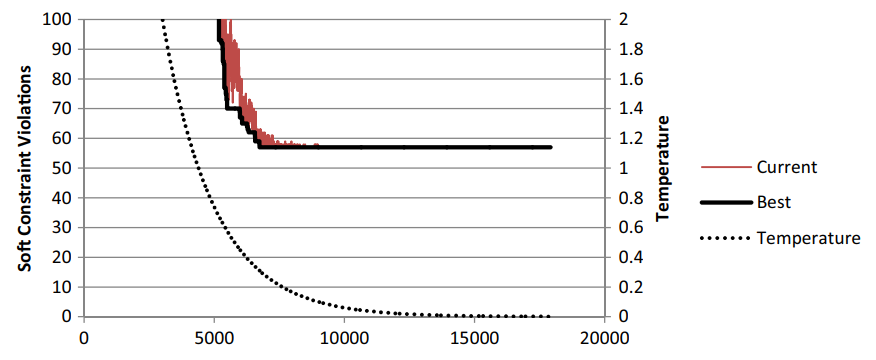
\includegraphics[width=0.5\textwidth]{images/related_works/SA/SAR_disabled.png}}
  \hfill
  \subfloat[Simulated Annealing with reheating enabled]{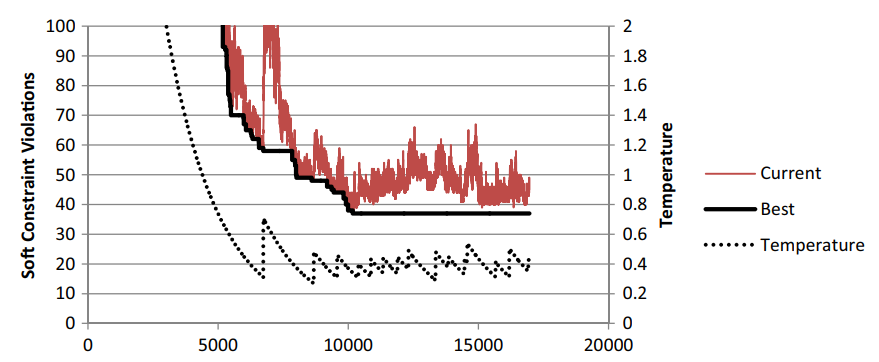
\includegraphics[width=0.5\textwidth]{images/related_works/SA/SAR_enabled.png}}
  \caption{Effect of reheating on the temperate and objective for Simulated Annealing as discovered by Leng Goh et al.\cite{Goh2017}}
  \label{fig:SAR}
\end{figure}


\subsubsection{Adaptive Large Neighbourhood Search}

Adaptive Large Neighbourhood Search \cite{ropke2006} works by generating new solutions by constantly making changes to the current solution in order to explore the neighbourhood space. These changes are obtained by removing part of the variables and then reintroducing new values in order to generate neighbours. Adaptive Large Neighbourhood Search is considered adaptive since it keeps track of the performance of used operations and adjusts its parameters accordingly. 

S{\o}rensen and Stidsen \cite{sorensen2012} propose a version of Adaptive Large Neighbourhood Search, building on the more general Large Neighbourhood Search algorithm. Large Neighbourhood Search works by creating new solutions by applying a "destroy" and "repair" operation. Every step, a destroy operation will remove a set of variables from the problem, before reintroducing new variables in order to create new solutions. By changing multiple variables, Large Neighbourhood Search is able to escape local minima. In the proposed Adaptive Large Neighbourhood Search extension however, the single destroy and repair operations are replaced by multiple operations, chosen at random during execution. This changes the original deterministic model into a stochastic version, introducing randomness. Additionally an adaptive layer analyses the impact of each operation and increases the probability of operations having a positive impact on the objective function.

\subsubsection{Great Deluge}

Dueck \cite{dueck1993} first proposed a Great Deluge algorithm as alternative to Simulated Annealing. It is built on the principle that the search space is limited by an ever changing water level. Newly generated solutions are only considered whenever they are superior compared to the objective threshold level that is represented by the water level. New solutions are found by performing low-level heuristics such as swapping two exams. While Dueck makes use of a simple linear function to determine the water level, different functions can be applied instead. While Simulated Annealing accepts worsening solutions based on a probabilistic value, Great Deluge has a hard cut-off point for accepting solutions. 

Burke et al. \cite{burke2004GD} are the first to apply an algorithm based on Great Deluge to the exam timetabling problem. Their reason for using Great Deluge is to be able to control the exact run time of the search while still allowing the search to converge. Although this could be done with the Simulated Annealing algorithm for example, determining the exact cooling rate for a correct execution time is often too complex. To solve this, they propose a Great Deluge implementation that they call a Degraded Ceiling algorithm. Instead of a changing water level, they describe a lowering ceiling with the ceiling representing the upper boundary of the objective function allowed. By slowly moving the ceiling down, the run time before convergence can be accurately determined. This is valuable for university administrators responsible for creating exam timetables since they could let the search run overnight or during the weekend.

By slowly lowering the ceiling, exploration to worsening solutions is feasible as long as the ceiling level has not cut off certain sections of the search space. As the ceiling lowers, the search space becomes tighter and priority shifts to exploitation. This continues until no further improvement is feasible and the stopping criterion is met. They conclude that this degraded ceiling implementation is not only superior to a time limited simulation annealing version, but that running this algorithm for long periods can produce extremely good results. Based on their analyses, degraded ceiling can outperform most algorithms whenever a long run time is feasible.

Kahar and Kendall \cite{kahar2015} propose a modified Great Deluge algorithm where the water level or decay rate is dynamically changed. Whenever no improvements are found, the change in water level can be reversed and the decay rate adjusted in order to allow for more exploration. Based on their analyses using data from Universiti Malaysia Pahang, the modified Great Deluge algorithm outperforms both the university's proprietary software and the original algorithm by Dueck \cite{dueck1993}. Lnasya Syafitrie and Komarudin \cite{Lnasya2022} implemented their own version based on this modified algorithm, with the main change being a slower rate at which the water rises. They find that their version outperforms that of Kahar and Kendall.

McMullan \cite{mcmullan2007} has implemented the Great Deluge algorithm with the addition of a reheating step, similar to the reheating used for Simulated Annealing with reheating \cite{Goh2017}. This better allows the search to escape local optima. While the general Great Deluge algorithm would terminate after observing no improvement for an amount of time steps, the proposed version will apply a one-time reheating, reducing the water level again. this allows certain worsening solutions to be accepted again, resulting in a larger possible share of the search space being visited. Afterwards, the decay rate is increased compared to the initial rate. Analyses using small, medium, and large benchmark data sets show that proposed Great Deluge algorithm outperforms other implementations such as Local Search and ant algorithms on the medium data sets. For the small and large data sets, no notable difference is noted.


\subsection{Population-based Meta-heuristics}
\subsubsection{Genetic Algorithms}

Genetic Algorithms \cite{Holland1975} are based on the process of natural selection witnessed in nature. It generally consists of several base steps before reaching a final solution. First, the algorithm creates an initial population consisting of feasible solutions. An iterative approach is then taken in order to evolve this population into new generations. For every generation, the fitness of each individual in the population is determined and the 'fittest' individuals are chosen as parents for the new generation. In order to obtain new offspring, genetic operators such as crossover and mutation are applied. Crossover works by combining information of parent solutions into a new offspring. This can be done by swapping exam assignments across the parents. Mutation on the other hand randomly changes assignments in order to create new offspring. This is done in order to maintain randomness, allowing Genetic Algorithms to escape local minima. The flow of the algorithm can be seen in Figure \ref{fig:GA}.

\begin{figure}[H]
	\centering
	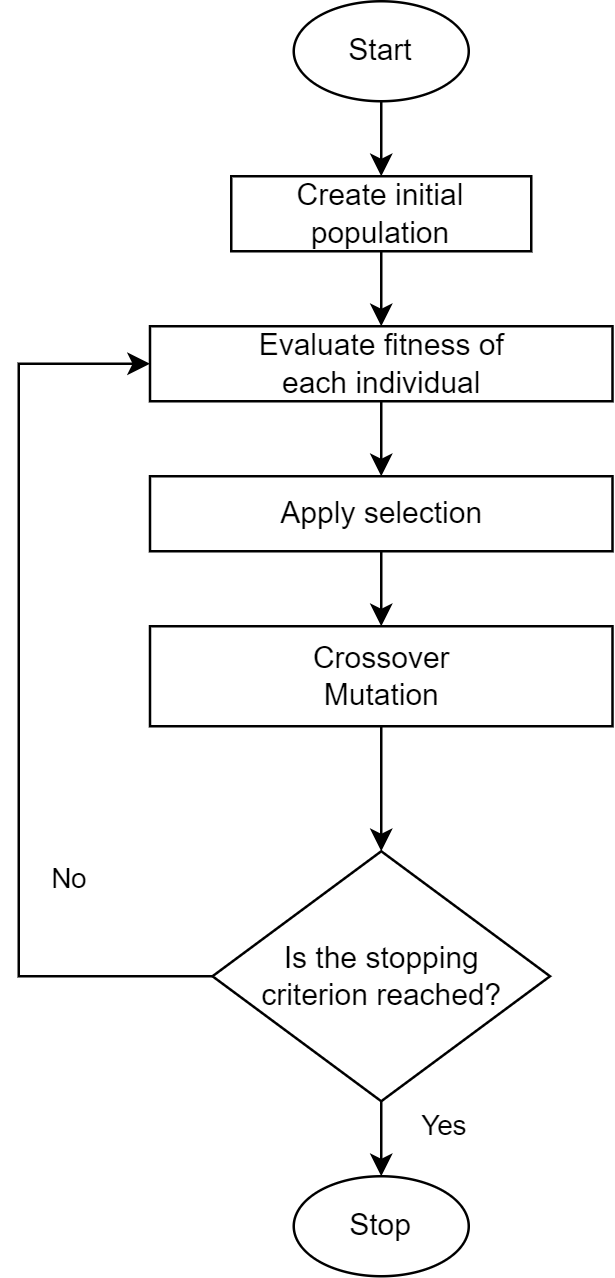
\includegraphics[width=0.40\textwidth]{images/related_works/GA/GA.png} 
	\caption{Genetic Algorithms flow}
	\label{fig:GA}
\end{figure}

The paper submitted by Pillay and Banzhaf \cite{pillay2010} showcases a two-phased approach to create feasible timetables. Both phases utilise a Genetic Algorithm implementation in order to come to a solution. While the first phase focuses on producing a timetable that does not violate any hard constraints, the second phase attempts to optimise the objective of the soft constraints. Up until 2007, most papers applying Genetic Algorithms used data sets specific to a particular institution. This algorithm is tested on the Carter benchmarks \cite{carter1996}, allowing its performance to be compared to different approaches.

During the first phase, domain specific heuristics are used instead of random operations in order to create the initial population. While these heuristics require domain knowledge, the quality of the initial population should be superior. In order to determine the next exam to be assigned, the obtained heuristics make use of the number of conflicts, the number of students enrolled per exam, or the number of students with conflicts. These heuristics were then compared to random and best-slot scheduling. It was found that using heuristics succeeded in lowering the soft constraints objective compared to other scheduling methods. For the iterative steps, the fitness function is described as the amount of conflicts per timetable. In order to select the parents with which to generate the new generation, tournament selection is applied. Here, a determined amount of individuals are randomly chosen from the population to be compared against each other. The individual having the lowest objective ends up being selected. This process is repeated until all parents have been selected. When creating new offspring, both mutation and crossover operators were considered. During mutation, a random amount of conflicting examinations are rescheduled. Moreover, crossover operations that randomly swap time slots between two parents were tested. This requires an additional repair mechanism to remove duplicate examinations and schedule missing examinations.
% TODO what to do about the last two sentences?

The second phase focuses on minimising the objective of the soft constraints in order the generate a more optimal timetable. While very similar to the first phase,  mutation operations are now continuously applied until an offspring superior to the parent is found, or a certain amount of iterations has been reached. The performance of this genetic algorithm was eventually compared to other studies using the same benchmark including Tabu Search and Large Neighbourhood Search. While no optimal solutions were found for any of the data sets, equal or improved solutions were obtained compared to alternative methods. They conclude that their implementation equals or even outperforms other evolutionary algorithms on the Carter benchmarks.

\subsubsection{Particle Swarm Optimisation}

Particle Swarm Optimisation \cite{kennedy1995} is derived from the behaviour by collective species as seen in fish schools and bird flocks. A swarm of particles (see fish or bird), representing solutions, moves through the search space at a certain speed and direction.
% TODO: expand on this?

Chen and Shih \cite{Chen2013} discuss a Particle Swarm Optimisation implementation combined with Local Search. During Particle Swarm Optimisation, a swarm of particles, with each particle corresponding to a different timetable, moves through the available search space. During every iteration, each particle will remember its best encountered position and share that information with the rest of the swarm. The particles will then adjust their velocity and direction on both their personal and global best. The velocity can be seen as the magnitude of the allowed change per time step. Additionally, a Local Search iteration is applied to explore the surrounding space for a better solution. In order to avoid particles being trapped in a local optimum, a disturbance operation is introduced \cite{tsai2010}. This operation forces particles to move towards unexpected directions, that aren't based on previous experience. 
% TODO data set

Tassopoulos and Beligiannis \cite{Tassopoulos2012} build on the general Particle Swarm Optimisation algorithm. Initially, they start with a high amount of 150 particles. Whenever the fitness value of a produced particle exceeds a certain tolerance value, this particle is set to inactive and will not be used in further steps. This tolerance value is calculated during each step in order to deactivate weak particles at the start, while making it harder for particles to reach that threshold down the line. When the amount of particles is reduced to 30, this procedure stops. The reasoning behind starting with a large amount of particles is to make it possible to explore a larger share of the search space, while keeping the execution time down by reducing the number of particles over time. Similar to Chen and Shih's approach \cite{Chen2013}, a Local Search algorithm is used to minimise one of the soft constraints. Results show that it outperforms the Genetic Algorithm implementation that their Particle Swarm Optimisation version was tested against.
% TODO data set
\subsubsection{Honey-Bee Mating Optimisation}

Honey-Bee Mating Optimisation \cite{abbas2001} is based on the mating of honey-bees as witnessed in nature. During the mating procedure, the queen representing the current best solution is able to mate with other bees in order to produce new solutions. Since specific terms, derived from the natural mating process, are used when describing the optimisation algorithm, Table \ref{tab:hbmo} provides translation of the analogy. Honey-Bee Mating Optimisation follows the natural process, during which the queen leaves the hive on a mating flight. She maintains a certain speed and direction, creating the possibility of drones to mate with her. After mating with a drone, its genetic information is stored within the queen to be used in the breeding phase. After each mating, the queen will change her energy level and speed. As soon as the queen reaches a certain energy threshold or reaches a mating limit, she will return to the hive. Upon return, the queen will randomly select genetic information obtained and perform a crossover step to create a new brood. Every brood is fed by a worker in order to improve the obtained solution. After every brood is improved, the fittest brood is compared to the queen. If the brood corresponds to a superior solution, the queen is replaced by the brood. Both the queen and the other broods are killed and a new mating flight will commence. 

Sabar et al. \cite{Sabar2009} are the first to propose the use of Honey-Bee Mating Optimisation in order to solve the exam timetabling problem. The proposed variant on the original algorithm \cite{abbas2001} attempts to solve its weakness of suffering from early convergence. Originally, the drones, that are used to mate with the queen, are never replaced which reduces the amount of variation. This is solved by replacing the drones that were successful in mating with the newly created broods. Additionally, after crossover, the heuristic applied by the worker is based on Local Search in order to optimise the brood as much as possible.

While Honey-Bee Mating Optimisation is very similar to other population based methods such as genetic algorithms, two clear differences can be noted. First, it maintains the queen as one of the two 'parents' used during crossover. Since the queen is considered as the current best solution, this is meant to improve obtained solutions. Secondly, the Local Search iteration applied by the worker can be considered an exploitation phase which is not present in Genetic Algorithms. Finally, Sabar et al. conclude that the proposed Honey-Bee Mating Optimisation alternative manages to create comparable or superior solutions compared against other population-based methods.

\begin{table}[H]
	\caption{Analogy between the natural mating process\\ and the Honey-Bee Mating Optimisation algorithm}
	\label{tab:hbmo}
	\centering
	\begin{tabular}{l c c }
		\hline
		\textbf{Natural honey bee}  & \textbf{Artificial honey bee} \\ \hline
		Queen & Current best solution \\
		Drones & Possible solutions \\
	    Broods & Newly generated solutions \\
            Worker & Heuristic search \\
            Mating or Breeding & Crossover \\ \hline
	\end{tabular}
\end{table}

% TODO data set

\subsection{Exact Methods}
\subsubsection{Integer Programming}

Kristiansen et al. \cite{kristiansen2015} describe a Mixed-Integer Programming model designed to solve XHSTT timetabling data sets. The XHSTT format was formulated to standardise timetabling data sets in order to compare heuristics. The proposed model makes use of two stages. During the first stage, a simplified Mixed-Integer Programming model is generated taking only the hard constraints of the problem into account. This stage is ran until a specified amount of time has passed or until the model has been solved to optimality. The benefit of using integer programming here is that Mixed-Integer Programming models can issue certificates of optimality, indicating that an optimal solution has been reached. This differs from heuristic methods where a model cannot guarantee that an optimal solution has been found unless the objective function is reduced to 0. With Mixed-Integer Programming models, one can determine whether the cost generated by the hard constraints is the most optimal solution feasible. This allows a clear cut off point for the model to stop focusing solely on the hard constraints. 

If a certificate of optimality can be generated, the second stage is executed. Otherwise, the algorithm ends. Before solving the model in stage 2, the soft constraints are added again. Additionally, an extra constraint is added, which keeps the optimal value of the cost generated by the hard constraints. The second stage ends when the remaining time after stage 1 has passed. The proposed model was not only successful in creating 2 new solutions to XHSTT data sets, it was also able to prove optimality of previously found solutions. Additionally, it could also provide the lower bounds for several other data sets and improve the best solution found so far. These lower bounds are crucial in order to compare the quality of solutions that have not reached optimality.
% TODO data set

Al-hawari et al. \cite{hawari2017} attempts to solve the university exam timetabling problem by splitting the problem into three smaller sub-problems. This allowed them to significantly decrease the amount of variables required in the formulas used, and thus reduce the processing power and storage capacity needed. Additionally, the simplification of the formulas improves the explainability of the model, making it easier to understand. The initial problem is split into 3 problems, each sub-problem continuing on the solution provided by the previous phase. Phase one and two will use a  graph colouring Integer Programming model to generate a feasible solution. Graph colouring works by assigning colours to the vertices while avoiding that two vertices connected by an edge are assigned the same colour. These vertices are called adjacent. Additionally, graph colouring will attempt to use the least amount of colours possible to generate a feasible solutions.

The first phase starts by assigning time slots to the different exams. Different from stated in the problem definition, Al-hawari et al. consider a time slot to be a moment in time when exams are being held. For example, during an exam period of 20 days with two exam moments a day, there would be 40 time slots available for exams to be planned. Initially, these time slots are solely an exam moment and do not include a day yet. During the first phase, exams are seen as the vertices with two vertices being connected by an edge if a student is enrolled in both exams. The time slots act as colours and are assigned to the vertices. Every feasible solution produced by this phase will satisfy the hard constraint that a student can not have more than one exam at the same time. Phase two builds upon this solution by assigning days to the time slots, meaning that the time slots are now considered vertices and the different days colours. Again, vertices are adjacent if the exams assigned to the time slots share mutual students. The new solution will have added the extra constraint that a student can't have two exams on the same day. Lastly, the third stage will assign all exams to rooms, keeping into account the exam enrolment and room capacity. The final solution, if feasible, will satisfy all hard constraints. An important remark to note is that no soft constraints were introduced for creating an improved exam distribution. As a result, a feasible solution will only make sure that a student has no exams on two following days or on the same day.
% TODO data set


\subsection{Hyper-heuristics}

While many optimisation methods have proven successful in generating optimal solutions, many of these methods are designed for a single problem and require domain-specific knowledge to be efficient. Hyper-heuristics attempt to solve this problem by providing a problem-independent solution which allows different methods to be used across problems. They can be considered either selective or generative. Selective hyper-heuristics choose from a predefined set of heuristics depending on the problem encountered, while generative hyper-heuristics procure new heuristics by combining multiple heuristics.

Kheiri and Keedwell \cite{kheiri2017} focus on the selection hyper-heuristics to solve the high school timetabling problem. Every iteration in the solution process consists of two steps. First, low-level heuristics are applied. These heuristic apply basic operations to create new solutions. Secondly, a move acceptance method will determine whether to keep or discard the new solution. In their study, a set of 15 low-level heuristics are employed including randomly rescheduling or unscheduling an exam, shuffling the time slots of several exams, changing the room of an exam, etc. For the move acceptance method, several methods such as Hill Climbing, Simulated Annealing and, Great Deluge are compared. The choice of acceptance method will determine whether a new solution is accepted. In hill climbing, a solution will only be accepted if its better compared to the previous solution. On the other hand, in Simulated Annealing, worse solutions can be considered due to the probability determined by the temperature.

The hyper-heuristic proposed by Kheiri and Keedwell makes use of sequence-based selection where each time a sequence of heuristics is applied instead of a single heuristic. Results show that these sequences outperform single applications of heuristics and that the selection of the low-level heuristics is more important than the move acceptance method used. Finally, they conclude that the proposed method provides solutions superior to those of previous popular methods.

Kendall and Mohd Hussin \cite{kendall2004} describe a hyper-heuristic where the order of the low-level heuristics applied to the current solution is determined by a Tabu Search implementation. At each step of the search, the heuristic with the best performance, if not tabu, is chosen to explore its own search space. Afterwards, the chosen heuristic becomes tabu, which means that it will not be considered in the next iterations. Because of this, the search space of other low-level heuristics that might perform worse will also be explored. The size of the tabu list becomes a variable to be optimised for each problem instance. The same set of 13 low-level heuristics proposed during one of their previous analyses was reused \cite{kendall2005}. Kendall and Mohd Hussin conclude that the hyper-heuristic is able to find solutions that are 80\% better compared to manual generated solutions based on their objective function.

\subsection{Method comparison}

To determine the search method to implement, we look at the following parameters for comparison:
\begin{description}
   \item [Research] \hfill \\ The amount of research performed for university examination timetabling. 
    \item [Parameters] \hfill \\ The amount of parameters to tune. The more parameters, the harder it is to determine an optimal set of parameters.
    \item [Explainability] \hfill \\ The explainability of the search method. The higher the explainability, the easier it is to explain the workings and interpret results.
    \item [Scalability] Due to a large data set, the scalability of the method is crucial in limiting the computational power and run time required.
\end{description}
 
\begin{table}[H]
	\caption{Comparison between the different algorithms}
	\label{tab:hbmo}
	\centering
	\begin{tabular}{l | c c c c c }
		\hline
		\textbf{Method}  & \textbf{Research} &\textbf{Parameters} &\textbf{Explainability}  & \textbf{Scalability}\\ \hline
		Tabu Search & +++ & + & +++ & +  \\
		Simulated Annealing & +++ & - & +++ & +  \\
	    Adaptive Large Neighbourhood Search &  - & -{}-{}- & - & -  \\
            Great Deluge & +++ & + & +++ & + \\
            Genetic Algorithms & +++& + & + & - \\ 
            Particle Swarm Optimisation & - & -{}-{}- & - & +++  \\ 
            Honey-Bee Mating Optimisation & - & -{}-{}-& - & -{}-{}- \\ 
            Integer Programming & + & - & - & +\\
            Hyper-heuristics & +++ & +++ & + & - \\
            \hline
	\end{tabular}
\end{table}
From this comparison, we have chosen to implement the Tabu Search algorithm. More precisely, the algorithm as proposed by Alvarez-Valdes et al. \cite{alvarez1997}, is used to conduct our analyses. Tabu Search has several positive qualities. First, the intuitive nature of Tabu Search improves the explainability of the method, which will ease the optimisation of the algorithm. Additionally, it also makes it easier to explain the method to the university administrators. Secondly, the tabu list prevents cycling between a set of states, which can reduce the amount of time needed to converge which will be crucial for the data sets provided. Finally, it has been shown that Tabu Search is able to outperform other competitive algorithms on data sets specific to institutions \cite{alvarez1997} \cite{colorni1999} \cite{Chu2000} as well as standardised benchmarks \cite{gaspero2001}.  